% Originally: content/week-02.tex, \subsection{Compact subsets} (Corsin Week 2, Friday)

\subsection{Compact subsets}

A subset $K$ of a metric space $(X,d)$ is compact if the metric space $(K, d|_{K \times K})$ is
compact (\cref{def:compact_metric_space}). This is equivalent to the definition in the script:

\begin{definition}[9.63, quoted from the official lecture notes]
\label{def:sequential_topological_compactness}
Let $(X,d)$ be a metric space. A subset $K \subset X$ is called \textbf{compact} if one of the
following equivalent conditions hold:
\begin{enumerate}[label=\textbf{(\alph*)}]
  \item \label{item:seq_compact_def963}
    $K$ is \textbf{sequentially compact}: every sequence $(x_n)_{n\in\mathbb{N}}$ in $K$ has
    a subsequence that is convergent (\cref{def:convergent_sequence}) in $K$.
  \item \label{item:top_compact_def963}
    $K$ is \textbf{topologically compact}: every family of open sets
    (\cref{def:open_closed}) $\{U_i\}_{i \in I}$ that cover $K$, has a finite subcover.
\end{enumerate}
\end{definition}

\begin{center}
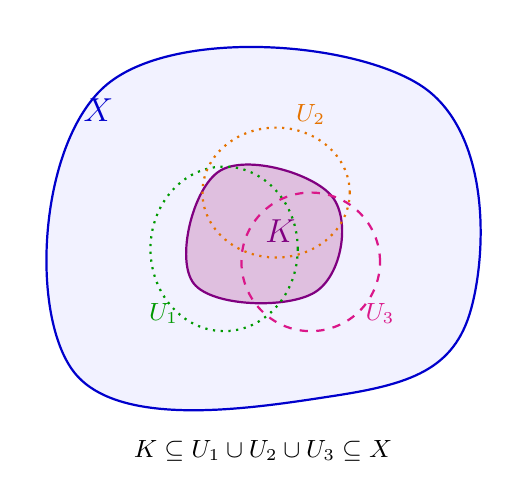
\begin{tikzpicture}[scale=1.1]
  \draw[blue!80!black, thick, fill=blue!5] plot[smooth cycle, tension=0.7] coordinates {(-2.2, -1.5) (-1.8, 1.8) (1.8, 1.8) (2.4, -0.8) (0.8, -1.8)};
  \node[blue!80!black, font=\large] at (-1.9, 1.5) {$X$};

  \draw[violet, thick, fill=violet!25] plot[smooth cycle, tension=0.7] coordinates {(-0.8, -0.5) (-0.5, 0.8) (0.8, 0.5) (0.6, -0.6)};
  \node[violet, font=\large] at (0.2, 0.1) {$K$};

  % As above: the three sets must cover all of K (they need not, and here do not,
  % cover all of X -- that is exactly the difference between the two pictures).
  \draw[green!60!black, thick, dotted] (-0.45,-0.1) ellipse (0.85 and 0.95);
  \node[green!60!black, font=\small] at (-1.15, -0.85) {$U_1$};

  \draw[orange!90!black, thick, dotted] (0.15,0.55) ellipse (0.85 and 0.75);
  \node[orange!90!black, font=\small] at (0.55, 1.45) {$U_2$};

  \draw[magenta!90!black, thick, dashed] (0.55,-0.25) ellipse (0.8 and 0.8);
  \node[magenta!90!black, font=\small] at (1.35, -0.85) {$U_3$};

  \node[below, font=\small] at (0, -2.2) {$K \subseteq U_1 \cup U_2 \cup U_3 \subseteq X$};
\end{tikzpicture}
\end{center}

% Quelle: Diego Torres Tejeda/Addendum - Sequential and Topological Compactness.pdf -- Sonnet 5 (Medium)
